%%%%%%%%%%%%%%%%%%%%%%%%%%%%%%%%%%%%%%%%%%%%%%%%%%%%%%%%%%%%%%%%%%%%%%%%%%%%%%%%%%
\begin{frame}[fragile]\frametitle{}

\begin{center}
{\Large NER with Bidirectional LSTM - CRF}

{\tiny (Ref:C omplete Tutorial on Named Entity Recognition (NER) using Python and Keras - by Akshay Chavan)}
\end{center}


\end{frame}


%%%%%%%%%%%%%%%%%%%%%%%%%%%%%%%%%%%%%%%%%%%%%%%%%%%%%%%%%%%%%%%%%%%%%%%%%%%%%%%%%%
\begin{frame}[fragile]\frametitle{NER}
NER is a method of extracting the relevant information from a large corpus and classifying those entities into predefined categories such as location, organization, name and so on. 
	
\begin{center}
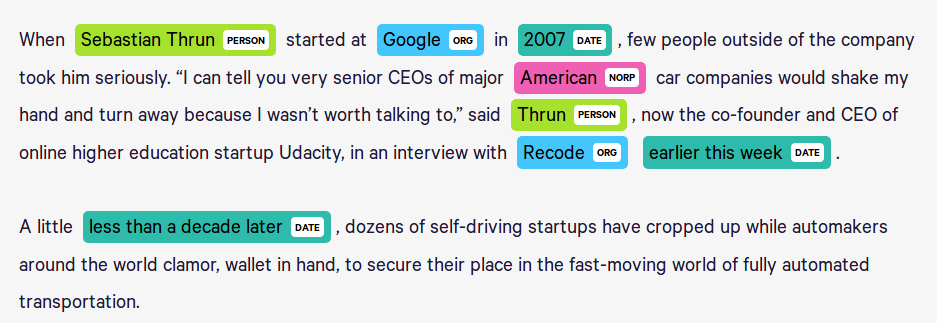
\includegraphics[width=0.8\linewidth,keepaspectratio]{spacy18}

	{\tiny (Ref: Complete Tutorial on Named Entity Recognition (NER) using Python and Keras - by Akshay Chavan)}

\end{center}

The conditional random field is used for predicting the sequences that use the contextual information to add information which will be used by the model to make correct predictions.

	{\tiny (Ref: Introduction to Conditional Random Fields (CRFs) - by Akshay Chavan)}

\end{frame}

%%%%%%%%%%%%%%%%%%%%%%%%%%%%%%%%%%%%%%%%%%%%%%%%%%%%%%%%%%%%%%%%%%%%%%%%%%%%%%%%%%
\begin{frame}[fragile]\frametitle{CRFs}
  \begin{itemize}
  \item To predict an output vector $y = {y_0, y_1, \ldots y_n}$ of a random variable given a feature vector $X$.
	\item The goal is to not only predict the output vector correctly but also the sequence of predictions matter a lot.
	\item The model predicts many variables that are interdependent.
	\item The main challenge behind the NER problem is that the entities that are too rare to appear in training set due to which model must identify based only on context. 
	\item The naive approach to this problem is to classify each word independently. 
	\item The main problem with this approach is it assumes that named entity labels are independent which is not the case.
	\item In CRFs where input data is sequence and output is also a sequence and we have to take the previous context into account when predicting on a data point.
  \end{itemize}
	

\end{frame}

%%%%%%%%%%%%%%%%%%%%%%%%%%%%%%%%%%%%%%%%%%%%%%%%%%%%%%%%%%%%%%%%%%%%%%%%%%%%%%%%%%
\begin{frame}[fragile]\frametitle{Understanding the data}

Source: https://www.kaggle.com/abhinavwalia95/entity-annotated-corpus having GMB(Groningen Meaning Bank) corpus which is tagged, annotated and built specifically to train the classifier to predict named entities such as name, location, etc. in BIO (or IOB) format where  B- denotes the beginning and I- inside of an entity. The words which are not of interest are labeled with 0 – tag.

\begin{lstlisting}
df = pd.read_csv('ner_dataset.csv', encoding = "ISO-8859-1")
print(df.head(10))
\end{lstlisting}


\begin{center}
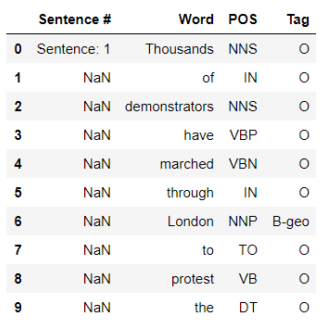
\includegraphics[width=0.4\linewidth,keepaspectratio]{spacy19}
\end{center}

\end{frame}

%%%%%%%%%%%%%%%%%%%%%%%%%%%%%%%%%%%%%%%%%%%%%%%%%%%%%%%%%%%%%%%%%%%%%%%%%%%%%%%%%%
\begin{frame}[fragile]\frametitle{Labels}
  \begin{itemize}
  \item geo = Geographical Entity
  \item org = Organization
  \item per = Person
  \item gpe = Geopolitical Entity
  \item tim = Time indicator
  \item art = Artifact
  \item eve = Event
  \item nat = Natural Phenomenon
  \end{itemize}
	

\end{frame}

%%%%%%%%%%%%%%%%%%%%%%%%%%%%%%%%%%%%%%%%%%%%%%%%%%%%%%%%%%%%%%%%%%%%%%%%%%%%%%%%%%
\begin{frame}[fragile]\frametitle{Understanding the data}


\begin{lstlisting}
df.describe()
\end{lstlisting}

\begin{center}
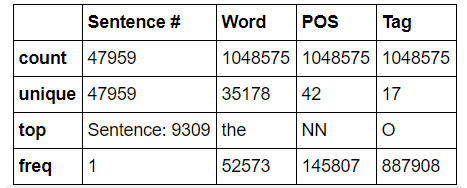
\includegraphics[width=0.35\linewidth,keepaspectratio]{spacy20}
\end{center}

\begin{lstlisting}
df['Tag'].unique()
array(['O', 'B-geo', 'B-gpe', 'B-per', 'I-geo', 'B-org', 'I-org', 'B-tim',
       'B-art', 'I-art', 'I-per', 'I-gpe', 'I-tim', 'B-nat', 'B-eve',
       'I-eve', 'I-nat'], dtype=object)
			 
df.isnull().sum()
Sentence #    1000616
Word                0
POS                 0
Tag                 0
\end{lstlisting}

  \begin{itemize}
  \item Total 47959 sentences and 17 labels.
  \item Number unique words in the dataset are 35178.
	\item Lots of missing values in 'Sentence \#' attribute.
  \end{itemize}
\end{frame}

%%%%%%%%%%%%%%%%%%%%%%%%%%%%%%%%%%%%%%%%%%%%%%%%%%%%%%%%%%%%%%%%%%%%%%%%%%%%%%%%%%
\begin{frame}[fragile]\frametitle{Preprocessing the data}

Populate sentences objects. Each will be list of tuples with its tag and pos.

\begin{lstlisting}
class sentence(object):
    def __init__(self, df):
        self.n_sent = 1
        self.df = df
        self.empty = False
        agg = lambda s : [(w, p, t) for w, p, t in zip(s['Word'].values.tolist(),
                                                       s['POS'].values.tolist(),
                                                       s['Tag'].values.tolist())]
        self.grouped = self.df.groupby("Sentence #").apply(agg)
        self.sentences = [s for s in self.grouped]
        
    def get_text(self):
        try:
            s = self.grouped['Sentence: {}'.format(self.n_sent)]
            self.n_sent +=1
            return s
        except:
            return None
\end{lstlisting}
\end{frame}

%%%%%%%%%%%%%%%%%%%%%%%%%%%%%%%%%%%%%%%%%%%%%%%%%%%%%%%%%%%%%%%%%%%%%%%%%%%%%%%%%%
\begin{frame}[fragile]\frametitle{Preprocessing the data}


\begin{lstlisting}
getter = sentence(df)
sent = getter.get_text()
print(sent)

[('Thousands', 'NNS', 'O'), ('of', 'IN', 'O'), ('demonstrators', 'NNS', 'O'), ('have', 'VBP', 'O'), ('marched', 'VBN', 'O'), ('through', 'IN', 'O'), ('London', 'NNP', 'B-geo'), ('to', 'TO', 'O'), ('protest', 'VB', 'O'), ('the', 'DT', 'O'), ('war', 'NN', 'O'), ('in', 'IN', 'O'), ('Iraq', 'NNP', 'B-geo'), ('and', 'CC', 'O'), ('demand', 'VB', 'O'), ('the', 'DT', 'O'), ('withdrawal', 'NN', 'O'), ('of', 'IN', 'O'), ('British', 'JJ', 'B-gpe'), ('troops', 'NNS', 'O'), ('from', 'IN', 'O'), ('that', 'DT', 'O'), ('country', 'NN', 'O'), ('.', '.', 'O')]

# Getting all the sentences in the dataset.
sentences = [" ".join([s[0] for s in sent]) for sent in getter.sentences]

\end{lstlisting}
\end{frame}

%%%%%%%%%%%%%%%%%%%%%%%%%%%%%%%%%%%%%%%%%%%%%%%%%%%%%%%%%%%%%%%%%%%%%%%%%%%%%%%%%%
\begin{frame}[fragile]\frametitle{Preprocessing the data}
Here word\_to\_index dictionary used to convert word into index value and tag\_to\_index is for the labels. So overall we represent each word as integer.

\begin{lstlisting}
#Getting unique words and labels from data
words = list(df['Word'].unique())
tags = list(df['Tag'].unique())
# Dictionary word:index pair
# word is key and its value is corresponding index
word_to_index = {w : i + 2 for i, w in enumerate(words)}
word_to_index["UNK"] = 1
word_to_index["PAD"] = 0

# Dictionary label:index pair
# label is key and value is index.
tag_to_index = {t : i + 1 for i, t in enumerate(tags)}
tag_to_index["PAD"] = 0

idx2word = {i: w for w, i in word_to_index.items()}
idx2tag = {i: w for w, i in tag_to_index.items()}
\end{lstlisting}
\end{frame}

%%%%%%%%%%%%%%%%%%%%%%%%%%%%%%%%%%%%%%%%%%%%%%%%%%%%%%%%%%%%%%%%%%%%%%%%%%%%%%%%%%
\begin{frame}[fragile]\frametitle{Preprocessing the data}

\begin{lstlisting}

print("The word India is identified by the index: {}".format(word_to_index["India"]))
print("The label B-org for the organization is identified by the index: {}".format(tag_to_index["B-org"]))

The word India is identified by the index: 2570
The label B-org for the organization is identified by the index: 6

# Converting each sentence into list of index from list of tokens
X = [[word_to_index[w[0]] for w in s] for s in sentences]

# Padding each sequence to have same length  of each word
X = pad_sequences(maxlen = max_len, sequences = X, padding = "post", value = word_to_index["PAD"])


# Convert label to index
y = [[tag_to_index[w[2]] for w in s] for s in sentences]

# padding
y = pad_sequences(maxlen = max_len, sequences = y, padding = "post", value = tag_to_index["PAD"])
\end{lstlisting}
\end{frame}

%%%%%%%%%%%%%%%%%%%%%%%%%%%%%%%%%%%%%%%%%%%%%%%%%%%%%%%%%%%%%%%%%%%%%%%%%%%%%%%%%%
\begin{frame}[fragile]\frametitle{Preparing Training data}

\begin{lstlisting}
num_tag = df['Tag'].nunique()
# One hot encoded labels
y = [to_categorical(i, num_classes = num_tag + 1) for i in y]
X_train, X_test, y_train, y_test = train_test_split(X, y, test_size = 0.15)

print("Size of training input data : ", X_train.shape)
print("Size of training output data : ", np.array(y_train).shape)
print("Size of testing input data : ", X_test.shape)
print("Size of testing output data : ", np.array(y_test).shape)

Size of training input data :  (40765, 75)
Size of training output data :  (40765, 75, 18)
Size of testing input data :  (7194, 75)
Size of testing output data :  (7194, 75, 18)
\end{lstlisting}
\end{frame}

%%%%%%%%%%%%%%%%%%%%%%%%%%%%%%%%%%%%%%%%%%%%%%%%%%%%%%%%%%%%%%%%%%%%%%%%%%%%%%%%%%
\begin{frame}[fragile]\frametitle{Preparing Training data}

\begin{lstlisting}
# Let's check the first sentence before and after processing.
print('*****Before Processing first sentence : *****\n', ' '.join([w[0] for w in sentences[0]]))
print('*****After Processing first sentence : *****\n ', X[0])

*****Before Processing first sentence : *****
 Thousands of demonstrators have marched through London to protest the war in Iraq and demand the withdrawal of British troops from that country .
*****After Processing first sentence : *****
  [ 2  3  4  5  6  7  8  9 10 11 12 13 14 15 16 11 17  3 18 19 20 21 22 23
  0  0  0  0  0  0  0  0  0  0  0  0  0  0  0  0  0  0  0  0  0  0  0  0
  0  0  0  0  0  0  0  0  0  0  0  0  0  0  0  0  0  0  0  0  0  0  0  0
  0  0  0]
\end{lstlisting}
\end{frame}

%%%%%%%%%%%%%%%%%%%%%%%%%%%%%%%%%%%%%%%%%%%%%%%%%%%%%%%%%%%%%%%%%%%%%%%%%%%%%%%%%%
\begin{frame}[fragile]\frametitle{Preparing Training data}

\begin{lstlisting}
# First label before and after processing.
print('*****Before Processing first sentence : *****\n', ' '.join([w[2] for w in sentences[0]]))
print('*****After Processing first sentence : *****\n ', y[0])

*****Before Processing first sentence : *****
 O O O O O O B-geo O O O O O B-geo O O O O O B-gpe O O O O O
*****After Processing first sentence : *****
  [[0. 1. 0. ... 0. 0. 0.]
 [0. 1. 0. ... 0. 0. 0.]
 [0. 1. 0. ... 0. 0. 0.]
 ...
 [1. 0. 0. ... 0. 0. 0.]
 [1. 0. 0. ... 0. 0. 0.]
 [1. 0. 0. ... 0. 0. 0.]]
\end{lstlisting}
\end{frame}


%%%%%%%%%%%%%%%%%%%%%%%%%%%%%%%%%%%%%%%%%%%%%%%%%%%%%%%%%%%%%%%%%%%%%%%%%%%%%%%%%%
\begin{frame}[fragile]\frametitle{Bidirectional LSTM-CRF Network}
\begin{lstlisting}
batch_size = 64 # Number of data points passed in each iteration
epochs = 8 # Passes through entire dataset
max_len = 75 # Maximum length of review
embedding = 40 # Dimension of embedding vector


num_tags = df['Tag'].nunique()
# Model architecture
input = Input(shape = (max_len,))
model = Embedding(input_dim = len(words) + 2, output_dim = embedding, input_length = max_len, mask_zero = True)(input)
model = Bidirectional(LSTM(units = 50, return_sequences=True, recurrent_dropout=0.1))(model)
model = TimeDistributed(Dense(50, activation="relu"))(model)
crf = CRF(num_tags+1)  # CRF layer
out = crf(model)  # output

model = Model(input, out)
model.compile(optimizer="rmsprop", loss=crf.loss_function, metrics=[crf.accuracy])
\end{lstlisting}
\end{frame}

%%%%%%%%%%%%%%%%%%%%%%%%%%%%%%%%%%%%%%%%%%%%%%%%%%%%%%%%%%%%%%%%%%%%%%%%%%%%%%%%%%
\begin{frame}[fragile]\frametitle{Bidirectional LSTM-CRF Network}
\begin{lstlisting}
model.summary()
_________________________________________________________________
Layer (type)                 Output Shape              Param #   
=================================================================
input_8 (InputLayer)         (None, 75)                0         
_________________________________________________________________
embedding_8 (Embedding)      (None, 75, 40)            1407200   
_________________________________________________________________
bidirectional_8 (Bidirection (None, 75, 100)           36400     
_________________________________________________________________
time_distributed_8 (TimeDist (None, 75, 50)            5050      
_________________________________________________________________
crf_8 (CRF)                  (None, 75, 18)            1278      
=================================================================
Total params: 1,449,928
Trainable params: 1,449,928
Non-trainable params: 0
\end{lstlisting}
\end{frame}

%%%%%%%%%%%%%%%%%%%%%%%%%%%%%%%%%%%%%%%%%%%%%%%%%%%%%%%%%%%%%%%%%%%%%%%%%%%%%%%%%%
\begin{frame}[fragile]\frametitle{Bidirectional LSTM-CRF Network}
Making Checkpoint each epoch to check and save the best model performance till last and also avoiding further validation loss drop due to overfitting.

\begin{lstlisting}
checkpointer = ModelCheckpoint(filepath = 'model.h5',
                       verbose = 0,
                       mode = 'auto',
                       save_best_only = True,
                       monitor='val_loss')
											 
history = model.fit(X_train, np.array(y_train), batch_size=batch_size, epochs=epochs,
                    validation_split=0.1, callbacks=[checkpointer])											 
\end{lstlisting}
\end{frame}

%%%%%%%%%%%%%%%%%%%%%%%%%%%%%%%%%%%%%%%%%%%%%%%%%%%%%%%%%%%%%%%%%%%%%%%%%%%%%%%%%%
\begin{frame}[fragile]\frametitle{Evaluation}

\begin{lstlisting}
history.history.keys()

dict_keys(['val_loss', 'val_crf_viterbi_accuracy', 'loss', 'crf_viterbi_accuracy'])
\end{lstlisting}

Visualizing the performance of model.
\begin{lstlisting}
acc = history.history['crf_viterbi_accuracy']
val_acc = history.history['val_crf_viterbi_accuracy']
loss = history.history['loss']
val_loss = history.history['val_loss']
plt.figure(figsize = (8, 8))
epochs = range(1, len(acc) + 1)
plt.plot(epochs, acc, 'bo', label='Training acc')
plt.plot(epochs, val_acc, 'b', label='Validation acc')
plt.title('Training and validation accuracy')
plt.legend()
\end{lstlisting}


\end{frame}

%%%%%%%%%%%%%%%%%%%%%%%%%%%%%%%%%%%%%%%%%%%%%%%%%%%%%%%%%%%%%%%%%%%%%%%%%%%%%%%%%%
\begin{frame}[fragile]\frametitle{Plot}
	
\begin{center}
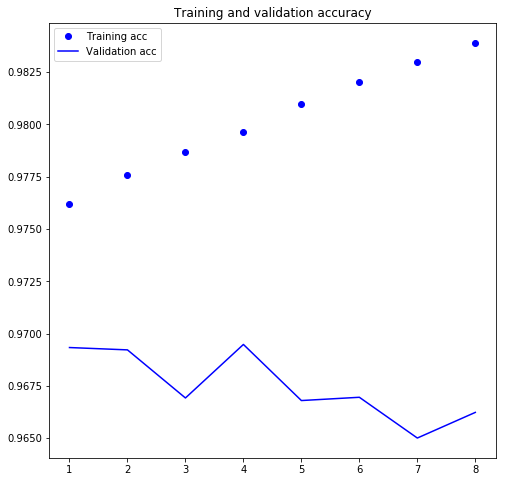
\includegraphics[width=0.6\linewidth,keepaspectratio]{spacy21}
\end{center}


\end{frame}

%%%%%%%%%%%%%%%%%%%%%%%%%%%%%%%%%%%%%%%%%%%%%%%%%%%%%%%%%%%%%%%%%%%%%%%%%%%%%%%%%%
\begin{frame}[fragile]\frametitle{Evaluation}

\begin{lstlisting}
# Evaluation
y_pred = model.predict(X_test)
y_pred = np.argmax(y_pred, axis=-1)
y_test_true = np.argmax(y_test, -1)

# Convert the index to tag
y_pred = [[idx2tag[i] for i in row] for row in y_pred]
y_test_true = [[idx2tag[i] for i in row] for row in y_test_true]
print("F1-score is : {:.1%}".format(f1_score(y_test_true, y_pred)))
F1-score is : 90.4%

\end{lstlisting}


\end{frame}

%%%%%%%%%%%%%%%%%%%%%%%%%%%%%%%%%%%%%%%%%%%%%%%%%%%%%%%%%%%%%%%%%%%%%%%%%%%%%%%%%%
\begin{frame}[fragile]\frametitle{Evaluation}

\begin{lstlisting}
report = flat_classification_report(y_pred=y_pred, y_true=y_test_true)
print(report)
             precision    recall  f1-score   support
      B-art       0.00      0.00      0.00        47
      B-eve       0.56      0.19      0.29        47
      B-geo       0.86      0.93      0.89      5632
      B-gpe       0.97      0.94      0.96      2418
      B-nat       0.00      0.00      0.00        30
      B-org       0.84      0.75      0.79      3001
      B-per       0.90      0.85      0.87      2562
      B-tim       0.93      0.90      0.91      3031
      I-art       0.00      0.00      0.00        27
      I-eve       0.00      0.00      0.00        40
      I-geo       0.80      0.86      0.83      1086
      I-gpe       1.00      0.52      0.68        25
      I-nat       0.00      0.00      0.00         6
      I-org       0.80      0.85      0.82      2436
      I-per       0.90      0.90      0.90      2626
      I-tim       0.86      0.74      0.80       941
          O       0.99      0.99      0.99    132279
        PAD       1.00      1.00      1.00    383316
avg / total       0.99      0.99      0.99    539550
\end{lstlisting}
\end{frame}

%%%%%%%%%%%%%%%%%%%%%%%%%%%%%%%%%%%%%%%%%%%%%%%%%%%%%%%%%%%%%%%%%%%%%%%%%%%%%%%%%%
\begin{frame}[fragile]\frametitle{Evaluation}

\begin{lstlisting}
# At every execution model picks some random test sample from test set.
i = np.random.randint(0,X_test.shape[0]) # choose a random number between 0 and len(X_te)b
p = model.predict(np.array([X_test[i]]))
p = np.argmax(p, axis=-1)
true = np.argmax(y_test[i], -1)

print("Sample number {} of {} (Test Set)".format(i, X_test.shape[0]))
# Visualization
print("{:15}||{:5}||{}".format("Word", "True", "Pred"))
print(30 * "=")
for w, t, pred in zip(X_test[i], true, p[0]):
    if w != 0:
        print("{:15}: {:5} {}".format(words[w-2], idx2tag[t], idx2tag[pred]))
\end{lstlisting}
\end{frame}

%%%%%%%%%%%%%%%%%%%%%%%%%%%%%%%%%%%%%%%%%%%%%%%%%%%%%%%%%%%%%%%%%%%%%%%%%%%%%%%%%%
\begin{frame}[fragile]\frametitle{Evaluation}

\begin{lstlisting}

Sample number 3435 of 7194 (Test Set)
Word           ||True ||Pred
==============================
It             : O     O
is             : O     O
the            : O     O
second         : O     O
major          : O     O
quarterly      : O     O
loss           : O     O
for            : O     O
Citigroup      : B-org B-org
,              : O     O
and            : O     O
:
earning        : O     O
reports        : O     O
over           : O     O
the            : O     O
past           : B-tim B-tim
week           : O     O
.              : O     O
\end{lstlisting}

Looks good!!
\end{frame}

